\section{Developments in \GAP infrastructure: Tools and processes for
  system and package development, quality assurance and release }\label{sec:gap-infra}

As well as developments in the core system and in packages, we have
dedicated considerable effort to improving our infrastructure and processes. 
In this section we describe developments in the technical processes
which support our developers (especially package developers),
connect them to our user community, and aim to 
ensure the robustness and quality of the integrated system.
\comment{Associated technical advocacy, training and support
were carried out through \GAP online support channels, as well 
as through development workshops reported in WP2 deliverables D2.2,
D2.11 and D2.15.}

\TODO{Think about the structure of this section -- at the moment it's
  not clear where it is going or what point is being made. Are we
  describing the overall situation, or developments made during \ODK}

\subsection{Regression testing}\label{testing}

\emph{Regression testing} is a software engineering technique which
checks (preferably in an automated way)
that new changes do not break functionality that 
worked previously. If a change breaks a test, that is 
a \emph{regression}. In \GAP, regressions may occur
when a change causes an incorrect result, or a crash, or an unwanted error
message; in addition, there may be \emph{performance regressions}
and \emph{memory regressions} where a test becomes slower, or uses
much more memory after a change.

Regression testing has been used by \GAP in one or another form since 
1980s, and by the start of \ODK, \GAP had established testing infrastructure
based on the private \href{https://jenkins.io/}{\sf Jenkins} installation
at USTAN, not accessible outside USTAN network. That was a major limiting
factor, because sharing tests outcomes with other developers and
allowing them to reproduce tests in the same environment was cumbersome
and required a lot of manual steps, requiring additional staff time.

%\GAP developers came to an understanding 
%that one of the limiting factors (not only for the testing, but for
%the \GAP development in general) was that while \GAP is an open source 
%software, it does not follow an open development model and does not
%have a public source code repository, and just before the start of
%the project established a public source code repository for \GAP
%on GitHub at \url{https://github.com/gap-system/gap}. 

%In the duration of the OpenDreamKit project we, together with other
%contributors to the \GAP project, consolidated \GAP development 
%around GitHub and its tool ecosystem.
%Hosting GAP repository on GitHub and eventual establishing of a number
%of other repositories under the gap-system and gap-packages 
%organizations (\url{https://github.com/gap-system} and 
%\url{https://github.com/gap-packages}), and encouraging package authors 
%to follow the same practices (see \url{https://gap-packages.github.io/})
%to find some further packages that are having public source code 
%repositories elsewhere) allowed us to bring our regression testing
%up to the next level.
%
%\TODO{maybe mention that we can break out onto GitLab if GitHub
%changes in some unacceptable way} 
%
\TODO{We need to get to this point much sooner. Can we reorder -- start with the
fact that instead of cumbersome manually maintained lists and whatever
the release manager now has modern dashbaords summarising lots of
stuff. Then explain how we got there and what all the components are?}

The widespread adoption of the open development model by the
developers of the \GAP system and especially package authors and
maintainers, occurring over the duration of \ODK, allowed \GAP
to substantially improve development workflows.
Today, anyone who is interested in checking the
status of the GAP test suite, can visit the public dashboard at
at \url{https://github.com/gap-system/gap-distribution/}, 
displayed on Figure~\ref{fig:gap-core-tests}.

The top part of Figure~\ref{fig:gap-core-tests} shows core system GAP tests,
which are run for every change made to the repository.
The ``status'' buttons lead to the test reports on the
public continuous integration platform \href{https://travis-ci.org/}{Travis CI}, and
the ``code coverage'' buttons lead to the public \href{https://codecov.io/}{Codecov} service
which produces the code coverage reports. Figure~\ref{fig:gap-core-tests} also
illustrated how the code coverage improved just over the last year,
since from 69\% in GAP 4.9.3 to 84\% in the master branch
(the prototype of the coming GAP~4.11 release). This level of testing
is achieved by the \GAP test 
suite for the core system consisting of a total of 707 test files at the time of writing
totaling over $60\,000$ lines,
as well as of the tests that check the correctness of over
over $14,000$ lines of 1810 manual examples.
%% \comment{1336 mansections containing examples;
%% 1641 (ref) + 169 (tut) = 1810 examples;
%% 13262 (ref) + 940 (tut) = 14202 lines}. 
%% in doc/ref
%Read("makedocreldata.g");
%exsref := ExtractExamples(GAPInfo.ManualDataRef.pathtodoc,
%       GAPInfo.ManualDataRef.main, GAPInfo.ManualDataRef.files, "Chapter");;
%exsref := Filtered( exsref, ch -> Length( ch ) > 0 );;
%Sum(List(exsref,Length));
%Sum(List(exsref, ch -> Sum(List( ch, ex -> Length(Filtered(SplitString(ex[1],"\n"), x -> x<>""))))));
%
%% in doc/tut
%Read("makedocreldata.g");
%exsref := ExtractExamples(GAPInfo.ManualDataTut.pathtodoc,
%       GAPInfo.ManualDataTut.main, GAPInfo.ManualDataTut.files, "Chapter");;
%exsref := Filtered( exsref, ch -> Length( ch ) > 0 );;
%Sum(List(exsref,Length));
%Sum(List(exsref, ch -> Sum(List( ch, ex -> Length(Filtered(SplitString(ex[1],"\n"), x -> x<>""))))));
%%
%% 
% and some further code in the {\tt benchmarks} directory. 
\TODO{Perhaps move the table with the number of lines in tests here, 
and also include code coverage in the table}
\GAP package authors are recommended to 
use a similar approach to testing and to provide their own regression
tests. Many do, adding, in total over a quarter of a million lines of
further tests.

\begin{figure}[!ht]
    \centering
    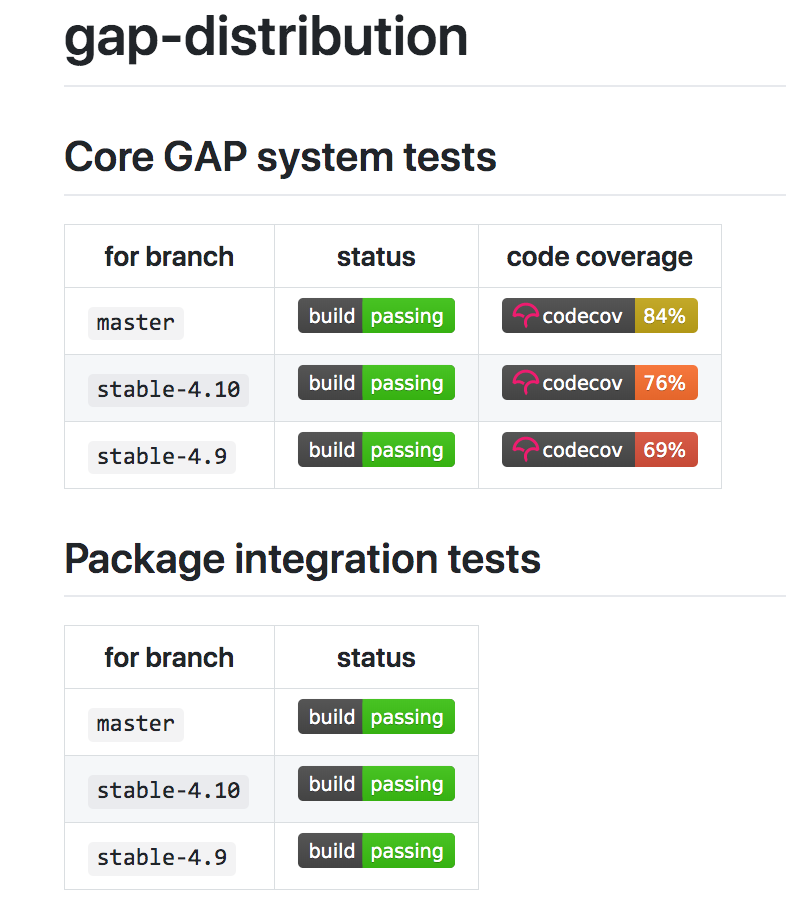
\includegraphics[width=5cm]{images/gap-core-tests}
    \caption{Dashboard with core GAP system and package integration tests}
    \label{fig:gap-core-tests}
\end{figure}

The bottom part of Figure~\ref{fig:gap-core-tests} shows the status 
of package integration tests
which are run once in 24 hours using a Docker container with
a snapshot of the GAP development version
and a selection of \GAP packages intended for the next release. 
Clicking on the ``status'' button leads to the overview displayed
on Figure~\ref{fig:gap-docker-master-testsuite}, from where one could inspect
test logs for each of the configurations. 

\begin{figure}[!ht]
    \centering
    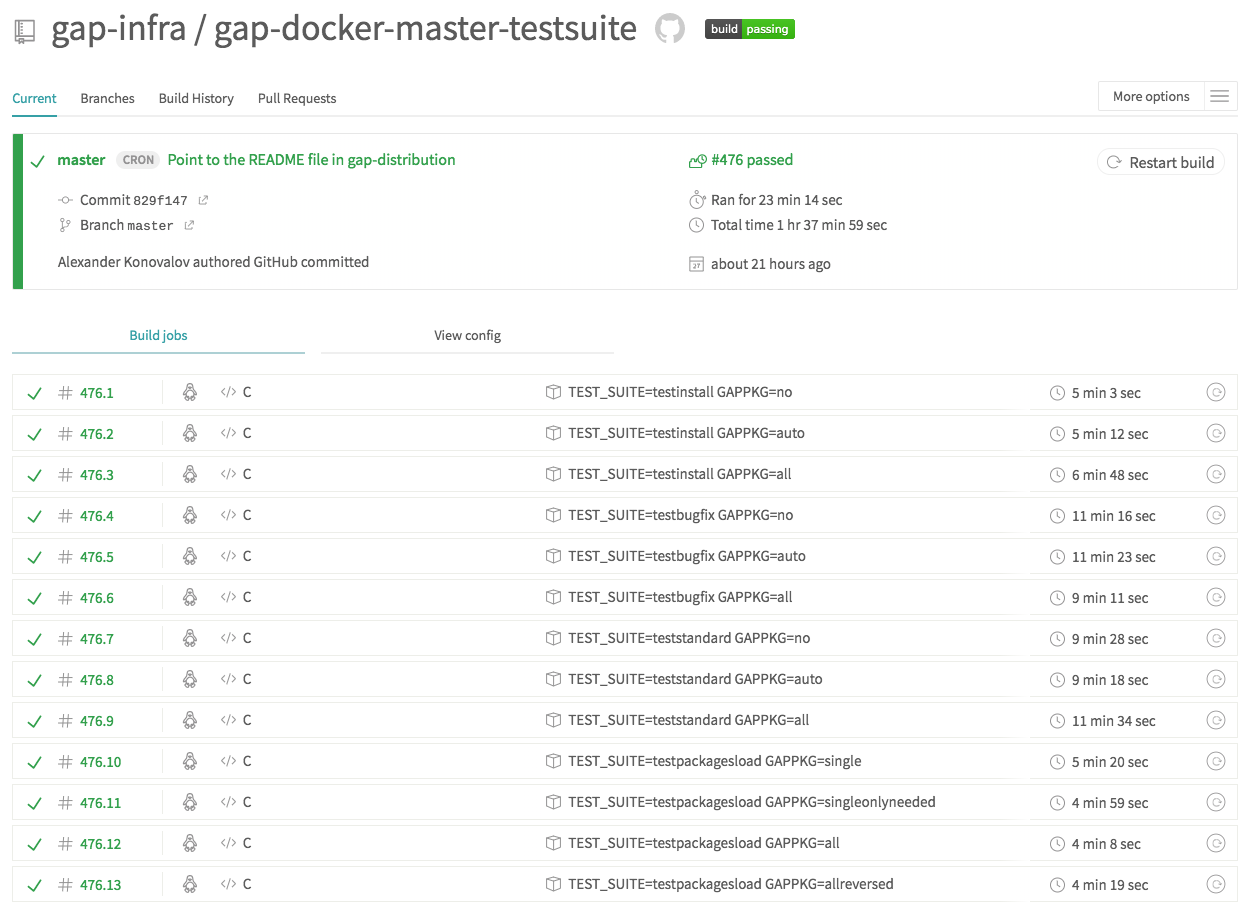
\includegraphics[width=\textwidth]{images/gap-docker-master-testsuite}
    \caption{GAP package integration tests on Travis CI}
    \label{fig:gap-docker-master-testsuite}
\end{figure}

At the same time, we continue to use Jenkins installation in USTAN 
for daily and weekly tests, running package updates system (Subsection~\ref{pkg-update}), wrapping and
testing release candidates (Subsection~\ref{distro}) and other automated tasks. It is also very valuable since 
it does not impose time limits on output inactivity and the overall duration
of the job; second, it allows us to log in into the test workspace for
debugging; third, with the specific \GAP setup for Windows we build it on a
machine with a Cygwin installation, and then install it on a clean Windows
machine to test there. 

\subsection{Docker containers for testing, using and sharing GAP code}

The Docker container for the test displayed on Figure~\ref{fig:gap-docker-master-testsuite}
is one of a set of containers that we maintain for various purposes, from offering 
them as alternative distributions (see Subsection~\ref{distro}) or components for sharable
reproducible experiments (see Appendix~\ref{sec:repro-gap}), to ways to speed up regression tests running
container-based tests on Travis CI. These containers are publicly available on Docker Hub
(see Figure~\ref{fig:gap-docker}).
\comment{The Docker stuff might deserve to be its own section}
\TODO{Refer to deliverable where Docker was previously reported}

\begin{figure}[!ht]
    \centering
    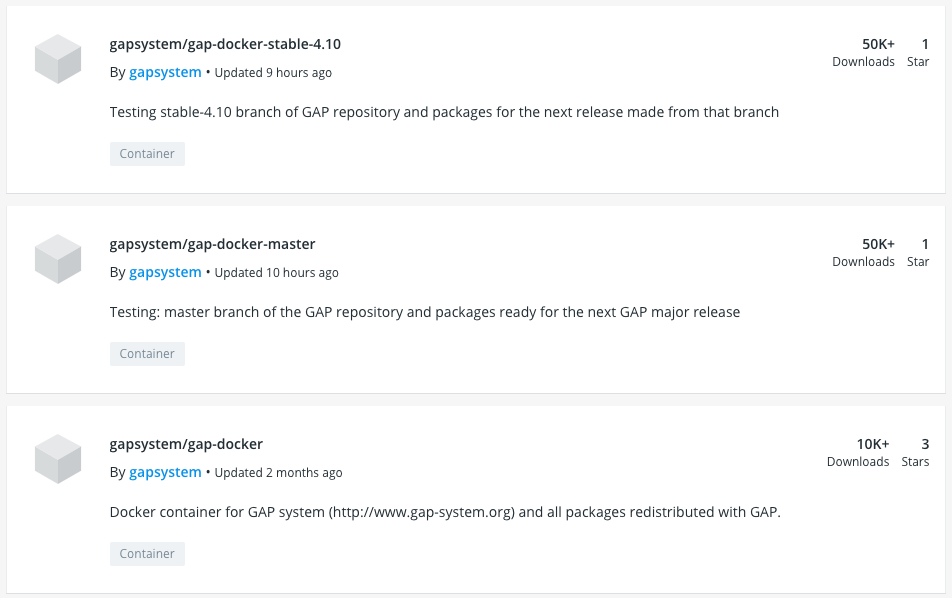
\includegraphics[width=12cm]{images/gap-docker}
    \caption{Selected \GAP Docker containers on Docker Hub}
    \label{fig:gap-docker}
\end{figure}

%We made use of \href{https://travis-ci.org/}{Travis CI} and
%\href{https://www.appveyor.com/}{AppVeyor} which are 
%free (for open source projects) continuous integration platforms 
%that can be used to build and test software projects hosted at GitHub.
%\emph{Continuous Integration}, usually abbreviated as {\bf CI} is the process
%automated building and testing for every performed or suggested changes to 
%the source code repository. Using Travis and AppVeyor, one can test changes proposed
%in a pull request \emph{before} they are merged into the main repository.
%At the moment, we use Travis CI for tests on Linux and OS X, and 
%AppVeyor for tests on Windows.

%In addition to that, we started to use \href{https://codecov.io/}{Codecov}
%platform to collect \emph{code coverage} reports for GAP to ensure that our
%regression tests exercise GAP codebase at an acceptable level, and then
%the changes which are submitted via pull request are actually being tested
%by Travis CI. Making these results easily obtainable and publicly available
%had a great effect on the community. Adding new tests to improve code coverage
%is a useful task for new contributors to familiarize themselves with the
%project setup. Making coverage reports available for each pull requests
%facilitates checking code coverage during code review and
%encourages their authors to ensure that their contributions have a good
%quality and their suggested changes are actually being tested. 




%%A crucial role in these developments was played by the enhanced
%%profiling facilities discussed 
%%in Subsection~\ref{gap-4.8}. 
%%GAP~4.8 also introduced the {\tt TestDirectory} function to find
%%(recursively) all {\tt .tst} files from a given directory or a list of 
%%directories and run them using {\tt Test}. Having ability to test
%%changes more efficiently also allowed us to further improve all 
%%tools involved in testing, making their output more informative,
%%and allowing test integration into various automated workflows
%%by a better detection of the test outcomes. 
% the logic seems backwards here. Better test tools let us test better, not v.v.
% What I had in mind was that once we set up the system with the
% state of the testing framework as it was, we were able to "test the testing"
% itself, and improve it - for example, by adding progress indicators,
% report time spent on GC and memory used, etc.




\subsection{Continuous Testing of Package Cross Compatibility Ahead of
\GAP Releases}\label{pkg-update}
For packages redistributed with \GAP, our automatic package update system
checks regularly for new versions on the authors web pages, retrieves them, and then uses them in a
number of checks to ensure that new package releases are compatible with
each other and do not break the functionality of the core \GAP system. The
same process also helps us to check that changes in the core \GAP system
do not break the functionality of the packages redistributed with \GAP.
%% (provided those packages have standard tests that allow us to do that
%% automatically)
This system has dramatically simplified the process of making a \GAP
release or update, for which we want a mutually compatible set of
package versions, also compatible with the new core system. This used
to require extensive negotiation with package authors, and sometimes
took months, even though the number of packages was much smaller. Now
developers have continuous visibility of the functionality and
compatibility of released and upcoming versions of packages and of the
core system, and releases are much faster.


\subsection{Packaging the \GAP distribution}\label{distro}

\TODO{Why are we talking about this here? Why does it relate to WP5,
  even tenuously}
\comment{See the Release checklist at \url{https://github.com/gap-system/gap-distribution/blob/master/DistributionUpdate/RELEASE_CHECKLIST.md}
Some text below pasted from there, needs shortening}

When there is a reasonable amount of changes in the core \GAP system
and/or sufficiently many package updates, and all the required
regression tests pass, we are considering publishing a new \GAP release
and offer it to the user community. It may be 
brought forward by crucial bugfixes or by highly demanded features;
in average we aim at making a minor release every several months 
and a major release once or twice per year. 
Figure~\ref{fig:gap-package-releases} shows the number of minor
and major \GAP releases per year, starting from the release of
\GAP~4.4 in 2004.

\begin{figure}[!ht]
    \centering
    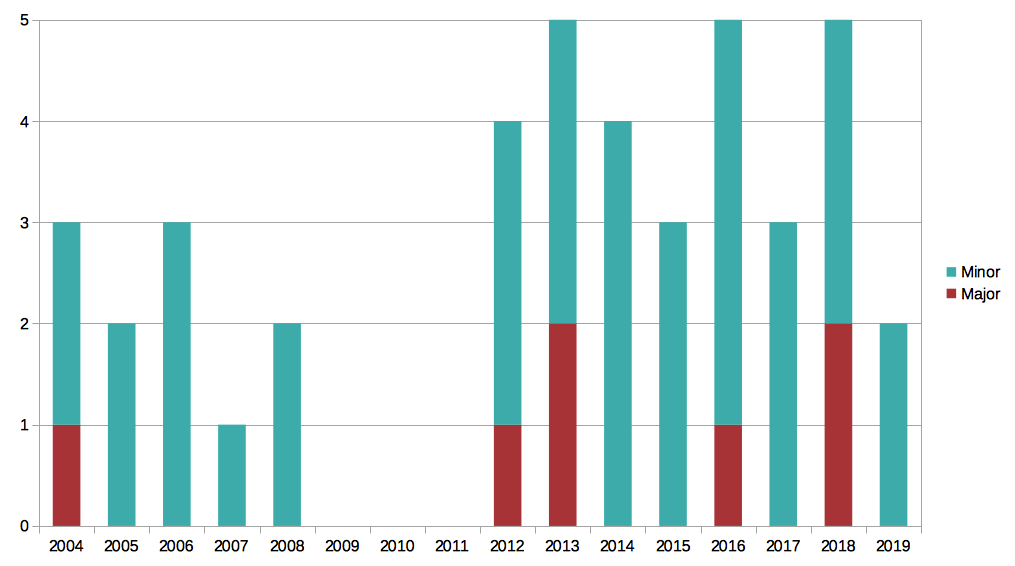
\includegraphics[width=\textwidth]{images/gap-releases}
    \caption{Number of major and minor \GAP releases per year since \GAP 4.4 release.}
    \label{fig:gap-releases}
\end{figure}

The use of the modern version control system such as {\sf Git}
helps us to have release branches and a master branch
where we accumulate changes planned for the next major release, and then
create the next release branch to stabilise the code and let package
authors to test it and if need be adapt their packages. That allowed
us to stop providing a beta release for package authors, starting from
\GAP~4.10.0. As noted in Subsection~\ref{gap-4.10},
enhanced automated regular testing permits us to concentrate on 
the changes in the master branch (a prototype of the next major release), and limit 
the changes in the current release branch to bugfixes and selected 
non-disruptive changes backported from the master branch.

Release wrapping and automated testing is performed in USTAN
using the Jenkins automation system. The \GAP distribution is tested
in various combinations of operating systems (Linux, macOS, Windows)
and build modes (32-bit and 64-bit), and with different sets of
loaded packages.
The \GAP distribution is provided in several archive formats for
Linux, macOS, and Windows,
and also as an executable installer for Windows.
We also provide several auxiliary archives used by providers of alternative
distributions, and systems which use \GAP (such as SageMath and OSCAR)
and for testing.
\GAP alternative distributions include the Docker container for the 
latest public \GAP release (\url{https://hub.docker.com/r/gapsystem/gap-docker/},
and a so called ``tap'' for the Homebrew package manager for OS x
(\url{https://github.com/gap-system/homebrew-gap}). 
It is also possible to try \GAP online in a Jupyter notebook running 
on Binder, following instructions from the README file in the repository
located at \url{https://github.com/gap-system/try-gap-in-jupyter}.
One could also use \GAP via a free or paid account
on \href{https://cocalc.com/}{\sf CoCalc} (formerly SageMathCloud).
The user should be aware that the combination of \GAP packages 
available there may differ from the one from the official \GAP distribution,
but it is possible to install additional packages under the user account
using the \GAP {\sf PackageManager} package (see Subsection~\ref{pkg-manager}).
